\documentclass[11pt]{article}
\usepackage[margin=1in]{geometry}
\usepackage{amsmath,amssymb,booktabs,array,graphicx,float,microtype}
\usepackage[authoryear]{natbib}
\usepackage[font=small,labelfont=bf]{caption}
\usepackage{xcolor}
\usepackage{hyperref}
\hypersetup{colorlinks=true,linkcolor=blue!55!black,citecolor=blue!55!black,urlcolor=blue!60!black}
\graphicspath{{output/}}
\newcommand{\DemandSD}{0.464}
\newcommand{\SupplySD}{0.670}
\newcommand{\FiscalResponseMonetary}{0.0086}
\newcommand{\MonetaryResponseFiscal}{0.0024}
\newcommand{\DemandMonetaryWedge}{0.00006}
\newcommand{\DemandFiscalWedge}{0.00001}
\newcommand{\SupplyMonetaryWedge}{0.00002}
\newcommand{\SupplyFiscalWedge}{0.00000}
\newcommand{\DemandFeedbackLoss}{0.2037}
\newcommand{\DemandOpenLoss}{0.2037}
\newcommand{\DemandCoopLoss}{0.2027}
\newcommand{\SupplyFeedbackLoss}{0.7078}
\newcommand{\SupplyOpenLoss}{0.7078}
\newcommand{\SupplyCoopLoss}{0.7074}
\newcommand{\StationaryRadius}{0.9383}
\newcommand{\DistinctStationary}{1}


\title{Policy as Strategic Investment:\\
A Recursive Monetary--Fiscal Game Calibrated to Australia}
\author{Monetary--Fiscal Coordination Project}
\date{26 September 2026}

\begin{document}
\maketitle

\begin{abstract}
This paper turns a two-stage monetary--fiscal policy game into a finite- and
infinite-horizon recursive game.  Instrument-adjustment costs are fixed
primitives.  Current monetary and fiscal choices instead constitute strategic
investments because they become payoff-relevant state variables and change the
other authority's later feedback action.  We solve the exact two-stage game by
backward induction, arbitrary finite horizons using coupled Riccati recursions,
a stationary Markov-perfect equilibrium, an open-loop Nash benchmark on the
identical economic system, and cooperation under a fixed social objective.
The model is calibrated using quarterly Australian transmission estimates.
The strategic channel is present: in the terminal subgame,
$\partial f_2/\partial m_1=\FiscalResponseMonetary$ and
$\partial m_2/\partial f_1=\MonetaryResponseFiscal$.  It is nevertheless small
at the baseline calibration.  Forty-quarter feedback Nash social losses are
\DemandFeedbackLoss\ after a demand contraction and \SupplyFeedbackLoss\
after a cost-push shock, compared with open-loop losses of \DemandOpenLoss\
and \SupplyOpenLoss.  The conclusion is substantive rather than computational:
adjustment costs make policy durable, but a large strategic-investment
distortion additionally requires strong cross-authority transmission and a
material conflict over the induced response.  The framework makes those
objects measurable and separates them from ordinary persistence and own-policy
smoothing.
\end{abstract}

\noindent\textbf{Keywords:} monetary--fiscal coordination; strategic
investment; Markov-perfect equilibrium; adjustment costs; policy games;
Australia.\\
\textbf{JEL codes:} E52, E58, E61, E62, C73.

\section{Introduction}

Monetary and fiscal policies affect the same output, inflation and debt
outcomes but need not be chosen by an authority with a common objective.  The
resulting interaction is not exhausted by a static Nash equilibrium.  A policy
choice made today can change the position inherited by tomorrow's policymakers
and thereby alter their incentives.  Current policy is then an investment in a
future strategic position.

The distinction matters for the interpretation of adjustment costs.  A term
such as $\lambda_M(m_t-m_{t-1})^2$ does not merely smooth the interest rate.
It makes $m_t$ part of tomorrow's state.  If fiscal policy responds to that
state, the monetary authority may move $m_t$ partly to influence future fiscal
policy.  The corresponding fiscal adjustment term creates the reciprocal
channel.  The adjustment coefficients $\lambda_M$ and $\lambda_F$ are
technological or institutional primitives in this paper; the authorities do
not choose their own objective coefficients.

This formulation follows the logic of strategic investment in industrial
organisation.  In \citet{Dixit1980} and \citet{FudenbergTirole1983}, a durable
first-stage choice commits a player to a position that changes a rival's
continuation behaviour.  \citet{FudenbergTirole1984} and
\citet{BulowEtAl1985} show that the sign of the distortion depends on two
distinct objects: whether the investment makes the player tough or soft, and
whether continuation actions are strategic complements or substitutes.
Adjustment costs provide durability in the present model, but they do not by
themselves determine either object.

Dynamic policy games apply closely related logic.  \citet{OudizSachs1984}
distinguish precommitment, time consistency, feedback and cooperation in
macroeconomic coordination.  \citet{Tabellini1986} studies monetary policy,
deficits and public debt in a dynamic linear--quadratic game.  Most directly,
\citet{BeetsmaBovenberg1997} treats public debt as a strategic fiscal state
that affects later monetary behaviour.  \citet{Gnocchi2013} demonstrates that
monetary--fiscal outcomes depend critically on the strategies to which the
central bank can commit.  These contributions imply that strategy space and
state definition are economic assumptions, not computational details.

The paper makes four contributions.  First, it supplies the exact backward-
induction extension of the original two-choice game.  Second, it decomposes the
stage-one first-order condition and identifies the rival-response term, rather
than labelling every continuation effect strategic.  Third, it compares
feedback and open-loop Nash equilibria on identical equations, shocks, weights
and adjustment costs.  Fourth, it documents convergence to a stationary
feedback equilibrium and conducts a multi-start numerical equilibrium search.

\section{The recursive Australian policy model}

\subsection{Economic block}

Let positive $m_t$ denote monetary tightening and positive $f_t$ denote a
fiscal expansion.  The empirical recursive block is
\begin{align}
 x_t &= \rho_x x_{t-1}+\sigma\pi_{t-1}-\sigma m_t+\psi f_t+d_t,
                                                        \label{eq:is}\\
 \pi_t &= \rho_\pi\pi_{t-1}+\kappa x_t+u_t,             \label{eq:pc}\\
 b_{t+1} &= \rho_b b_t+\chi_m m_t+\chi_f f_t-\chi_\pi\pi_t,
                                                        \label{eq:debt}\\
 d_{t+1}&=\rho_d d_t+\varepsilon^d_{t+1},\qquad
 u_{t+1}=\rho_u u_t+\varepsilon^u_{t+1}.                \label{eq:shocks}
\end{align}
The policy state before decisions at $t$ is
\begin{equation}
 s_t=(x_{t-1},\pi_{t-1},b_t,m_{t-1},f_{t-1},d_t,u_t)'.   \label{eq:state}
\end{equation}
Equations \eqref{eq:is}--\eqref{eq:shocks} can be collected as
\begin{equation}
 s_{t+1}=A s_t+B_Mm_t+B_Ff_t+\varepsilon_{t+1}.          \label{eq:transition}
\end{equation}
The unit entries in $B_M$ and $B_F$ place the current instruments in the next
period's lagged-instrument states.  They are the formal link between the
two-stage game and its dynamic extension.

The block is deliberately transparent.  The output and inflation equations
are hybrid, backward-looking empirical relations rather than the fully
forward-looking New Keynesian IS and Phillips curves.  This permits an exact
recursive solution and a clean comparison of equilibrium concepts.  It also
sets a boundary on interpretation: the exercise does not yet incorporate the
additional commitment channel operating through private expectations.

\subsection{Agency mandates and true social welfare}

Authority $j\in\{M,F\}$ minimizes
\begin{align}
 L_j=E_0\sum_{t=0}^{T-1}\beta_j^t\big[&
 \omega^j_\pi\pi_t^2+\omega^j_xx_t^2+\omega^j_bb_{t+1}^2
 +\omega^j_m m_t^2+\omega^j_f f_t^2 \nonumber\\
 &+\lambda^j_M(m_t-m_{t-1})^2
 +\lambda^j_F(f_t-f_{t-1})^2\big].                    \label{eq:loss}
\end{align}
The central bank places greater relative weight on inflation; the fiscal
authority places greater relative weight on output.  These weights are held
fixed across every solution concept.

Cooperation minimizes a third loss $L_S$ of the same form.  It represents true
social welfare and is not the sum of the two institutional mandates.  This
separation prevents the definition of cooperation from changing whenever the
agencies' delegated objectives change.

In matrix form, the stage loss is
\begin{equation}
 \ell_j(s_t,m_t,f_t)=
 \begin{bmatrix}s_t'&m_t&f_t\end{bmatrix}
 Q_j
 \begin{bmatrix}s_t'&m_t&f_t\end{bmatrix}'.             \label{eq:qform}
\end{equation}

\section{Strategic investment and equilibrium concepts}

\subsection{The exact two-stage game}

At stage 2, the two authorities play a simultaneous Nash game conditional on
$s_2$.  Its linear decision rules are
\begin{equation}
 m_2=K_{M,2}s_2,\qquad f_2=K_{F,2}s_2.                  \label{eq:terminalrules}
\end{equation}
At stage 1, each authority understands that its action changes $s_2$ and hence
both rules in \eqref{eq:terminalrules}.  For the monetary authority,
\begin{equation}
 0=\ell^M_{m_1}+\beta_M B_M'\nabla V^M_2(s_2).          \label{eq:stage1foc}
\end{equation}
Using the terminal monetary first-order condition gives the envelope
decomposition
\begin{equation}
 \nabla V^M_2=
 \underbrace{\ell^M_{s_2}}_{\text{direct state effect}}
 +\underbrace{K_{F,2}'\ell^M_{f_2}}_{\text{rival-response effect}}. \label{eq:decomp}
\end{equation}
The term $K_{M,2}'\ell^M_{m_2}$ vanishes by the monetary authority's own
terminal first-order condition.  Therefore
\begin{equation}
 \mathcal S_M=\beta_M B_M'K_{F,2}'\ell^M_{f_2}           \label{eq:sm}
\end{equation}
is the monetary strategic-investment wedge.  Similarly,
\begin{equation}
 \mathcal S_F=\beta_F B_F'K_{M,2}'\ell^F_{m_2}.          \label{eq:sf}
\end{equation}
This isolates the strategic term from own adjustment costs, ordinary macro
persistence and debt dynamics.  Strategic investment exists only if the
current policy changes the rival's later action and that action matters for
the current policymaker's loss.

\subsection{Finite-horizon feedback Nash}

Suppose the continuation values are quadratic,
$V^j_{t+1}(s)=s'P^j_{t+1}s$.  At each date the simultaneous policy first-order
conditions are
\begin{equation}
 \begin{bmatrix}
 Q^M_{mm}+\beta_M B_M'P^M_{t+1}B_M &
 Q^M_{mf}+\beta_M B_M'P^M_{t+1}B_F\\
 Q^F_{fm}+\beta_F B_F'P^F_{t+1}B_M &
 Q^F_{ff}+\beta_F B_F'P^F_{t+1}B_F
 \end{bmatrix}
 \begin{bmatrix}m_t\\f_t\end{bmatrix}
 =-
 \begin{bmatrix}
 Q^M_{ms}+\beta_M B_M'P^M_{t+1}A\\
 Q^F_{fs}+\beta_F B_F'P^F_{t+1}A
 \end{bmatrix}s_t.                                     \label{eq:coupled}
\end{equation}
Solving \eqref{eq:coupled} yields $K_{M,t}$ and $K_{F,t}$.  With
$A_t^c=A+B_MK_{M,t}+B_FK_{F,t}$, each value matrix is updated by
\begin{equation}
 P^j_t=S_t'Q_jS_t+\beta_j(A_t^c)'P^j_{t+1}A_t^c,
 \quad
 S_t=\begin{bmatrix}I\\K_{M,t}\\K_{F,t}\end{bmatrix}. \label{eq:riccati}
\end{equation}
Starting from $P^j_{T+1}=0$ and working backwards produces a subgame-perfect
feedback Nash equilibrium.  For $T=2$, this is exactly the original two-stage
logic.  As $T$ grows, the initial rules converge to a stationary coupled-
Riccati fixed point.

\subsection{Open loop, cooperation and equilibrium selection}

In the open-loop Nash benchmark, both authorities select complete paths at
date zero.  Later controls therefore do not respond to a deviation that changes
an inherited state.  We solve this game by stacking \eqref{eq:transition} and
the quadratic losses, not by changing the economy.  The difference between
feedback and open loop consequently identifies the value of state-contingent
continuation behaviour in this calibration.

The cooperative regulator uses the same backward recursion but chooses both
instruments to minimize $L_S$.  Finally, the stationary Nash solution is
computed from several dispersed initial value matrices.  Finding the same
stabilising fixed point from these starts is useful evidence, but is not a
mathematical proof that no other Markov-perfect equilibrium exists.

\section{Australian calibration}

The quarterly output and inflation equations use the 1993Q1--2019Q4
Australian estimates employed in the companion model.  The cached source data
come from the Reserve Bank of Australia's statistical tables.  The debt block
and loss weights are transparent calibrations rather than structural
estimates.  Table \ref{tab:calibration} reports the principal values.

\begin{table}[H]
\centering
\caption{Baseline calibration}
\label{tab:calibration}
\begin{tabular}{lll}
\toprule
Parameter & Value & Interpretation\\
\midrule
$\rho_x$ & 0.62875 & output-gap persistence\\
$\rho_\pi$ & 0.56255 & inflation persistence\\
$\sigma$ & 0.03695 & monetary transmission to output\\
$\psi$ & 0.05142 & fiscal transmission to output\\
$\kappa$ & 0.15511 & Phillips slope\\
$\rho_b$ & 0.995 & debt persistence\\
$(\chi_m,\chi_f,\chi_\pi)$ & $(0.015,0.060,0.100)$ & debt transmission\\
$(\lambda_M,\lambda_F)$ & $(0.050,0.040)$ & primitive adjustment weights\\
$(\omega^M_\pi,\omega^M_x)$ & $(1.50,0.25)$ & monetary mandate\\
$(\omega^F_\pi,\omega^F_x)$ & $(0.50,0.75)$ & fiscal mandate\\
$(\omega^S_\pi,\omega^S_x)$ & $(1.00,0.50)$ & social objective\\
\bottomrule
\end{tabular}
\end{table}

The experiments use a one-standard-deviation demand contraction of
$\DemandSD$ and a cost-push innovation of $\SupplySD$.  Innovations after the
initial impulse are zero in the plotted paths.  Under linear--quadratic
certainty equivalence, additive shock variances affect expected loss but not
the policy gains.  Persistent shocks could be included by changing $\rho_d$
and $\rho_u$ without altering the solution method.

\section{Results}

\subsection{The two-stage mechanism is present but small}

Table \ref{tab:twostage} reports the exact stage-2 response coefficients and
the realised strategic component of the stage-1 half-gradient.  The two cross
responses are positive under the sign convention used here.  A monetary
tightening today raises the fiscal expansion chosen in the continuation game;
a fiscal expansion today raises subsequent monetary tightening.  The policy
positions are therefore locally complementary in this cross-stage sense.

\begin{table}[H]
\centering
\caption{Two-stage strategic-investment diagnostics}
\label{tab:twostage}
\begin{tabular}{lrr}
\toprule
Diagnostic & Demand contraction & Cost-push shock\\
\midrule
$\partial f_2/\partial m_1$ & 0.00856 & 0.00856\\
$\partial m_2/\partial f_1$ & 0.00237 & 0.00237\\
Monetary strategic wedge $\mathcal S_M$ & 0.000055 & 0.000021\\
Fiscal strategic wedge $\mathcal S_F$ & 0.000011 & 0.000004\\
Monetary total continuation derivative & 0.002173 & $-0.003395$\\
Fiscal total continuation derivative & $-0.005328$ & 0.001140\\
\bottomrule
\end{tabular}
\end{table}

The signs establish the mechanism; their scale disciplines its interpretation.
For the demand shock, the monetary strategic term is about 2.6 per cent of the
absolute monetary continuation derivative.  The fiscal share is roughly 0.2
per cent.  The remaining continuation incentive comes from direct macro
persistence, debt and own-policy smoothing.  Thus it would be incorrect to
call the entire continuation term strategic investment.

Figure \ref{fig:two} compares feedback and open-loop policies in the exact
two-stage experiment.  Their difference is visible numerically but small.
This is not a failure of backward induction: it is the implication of weak
estimated instrument transmission and small cross-stage response slopes.

\begin{figure}[H]
\centering
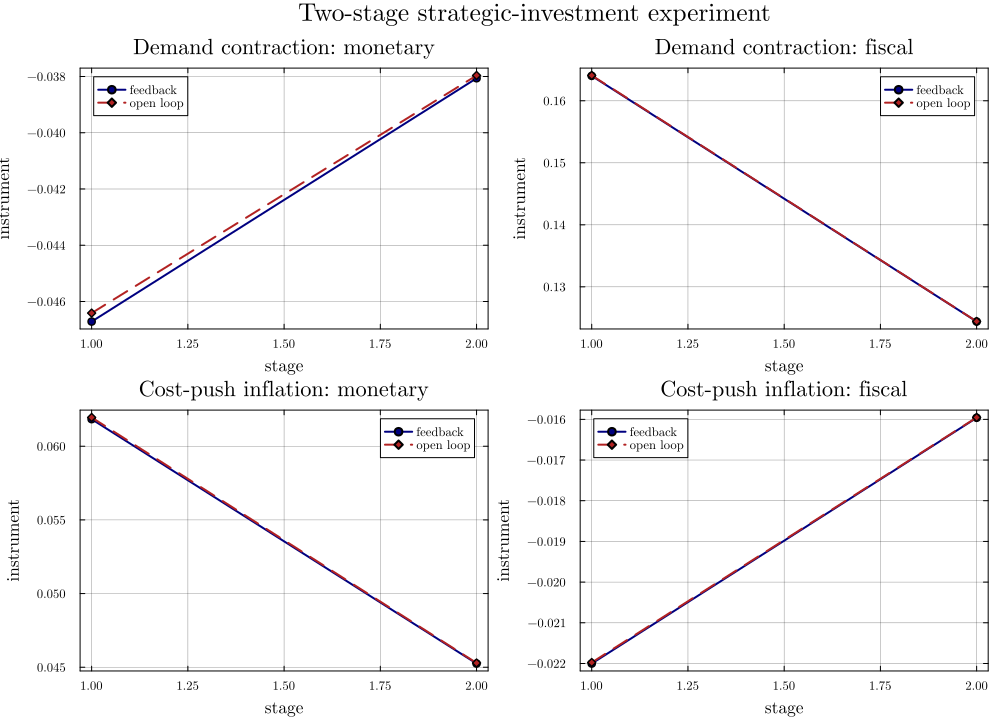
\includegraphics[width=0.92\textwidth]{two_stage_policies.png}
\caption{Exact two-stage feedback and complete-path open-loop policies.}
\label{fig:two}
\end{figure}

\subsection{The dynamic solution}

Table \ref{tab:dynamic} reports forty-quarter losses.  Feedback Nash and open
loop are close under both shocks.  Cooperation matters more, especially for
the allocation of instruments, but even its welfare gain is modest at this
local calibration.

\begin{table}[H]
\centering
\caption{Forty-quarter social loss}
\label{tab:dynamic}
\begin{tabular}{lrr}
\toprule
Regime & Demand contraction & Cost-push shock\\
\midrule
Feedback Nash & \DemandFeedbackLoss & \SupplyFeedbackLoss\\
Open-loop Nash & \DemandOpenLoss & \SupplyOpenLoss\\
Cooperation & \DemandCoopLoss & \SupplyCoopLoss\\
Stationary MPE rule & 0.2037 & 0.7079\\
\bottomrule
\end{tabular}
\end{table}

Figures \ref{fig:demand} and \ref{fig:supply} show the corresponding impulse
responses.  The stationary MPE and the forty-period feedback solution nearly
coincide at the beginning of the sample.  Open loop is also close, consistent
with the small strategic wedges.  Cooperation uses a different policy mix:
following a demand contraction it relies relatively more on monetary easing
and less on fiscal expansion.

\begin{figure}[H]
\centering
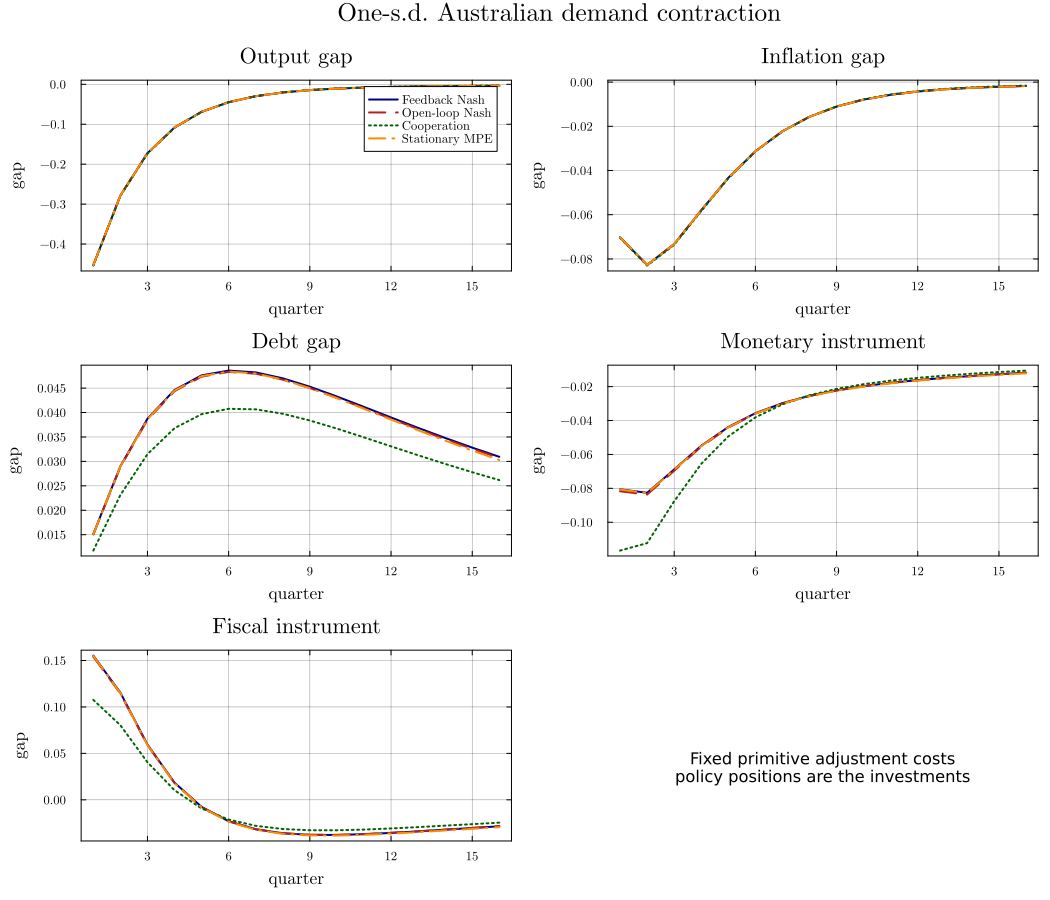
\includegraphics[width=0.94\textwidth]{dynamic_demand_irfs.png}
\caption{Dynamic responses to a one-standard-deviation Australian demand contraction.}
\label{fig:demand}
\end{figure}

\begin{figure}[H]
\centering
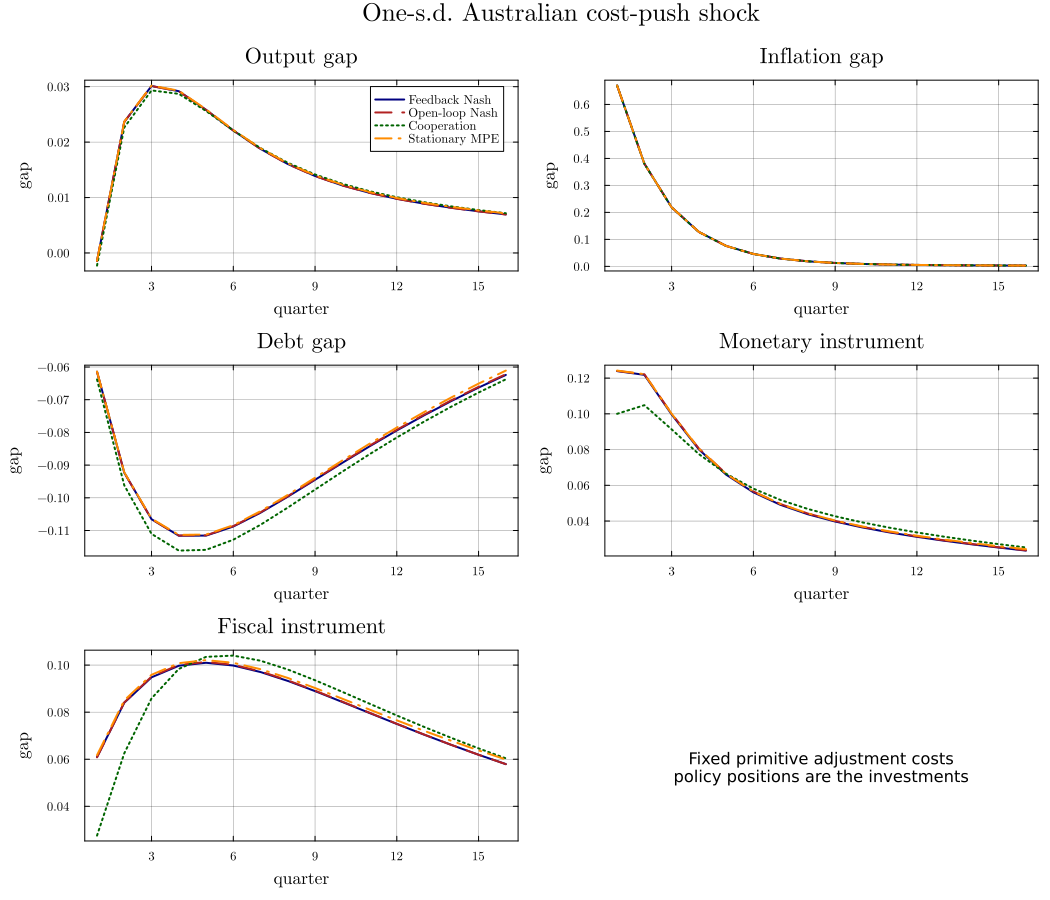
\includegraphics[width=0.94\textwidth]{dynamic_cost_push_irfs.png}
\caption{Dynamic responses to a one-standard-deviation Australian cost-push shock.}
\label{fig:supply}
\end{figure}

\subsection{Horizon convergence and stationary equilibrium}

The finite-horizon rule converges steadily toward the stationary feedback
rule.  At horizon 40 its Euclidean coefficient distance is 0.00534; at horizon
80 it is $2.1\times10^{-5}$.  The stationary closed-loop spectral radius is
\StationaryRadius, so the selected equilibrium is locally stable.

Six Riccati initialisations ranging from zero to one hundred times the stage-
loss state matrix all converged to the same rule to numerical tolerance.  The
search therefore found \DistinctStationary\ distinct stable solution.  This is
reassuring for the baseline but should not be read as a global uniqueness
theorem.  If stronger complementarity creates multiple fixed points, they
should be sought using continuation methods and direct solution of the coupled
algebraic equations.

\begin{figure}[H]
\centering
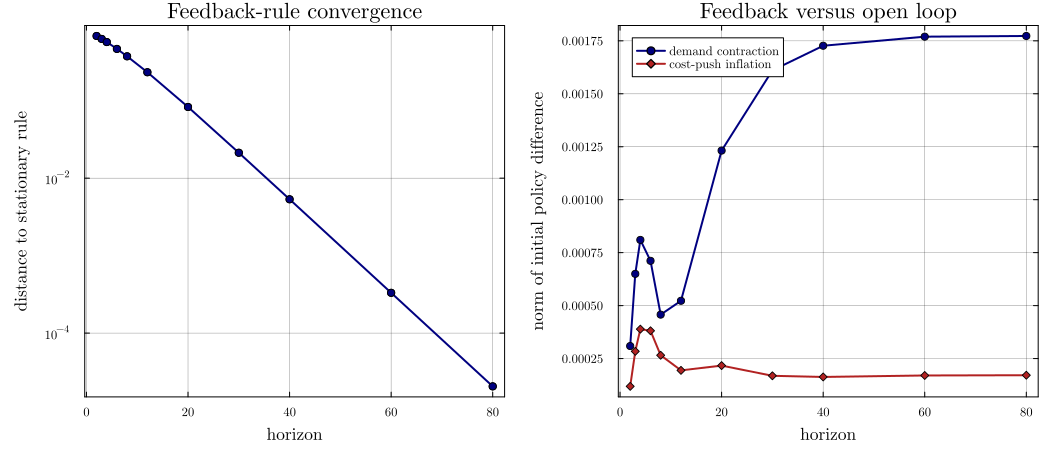
\includegraphics[width=0.94\textwidth]{horizon_convergence.png}
\caption{Convergence to the stationary feedback rule and the feedback--open-loop gap.}
\label{fig:horizon}
\end{figure}

\subsection{Why larger adjustment costs do not automatically create a large game}

Figure \ref{fig:sensitivity} scales both primitive adjustment-cost weights
while holding structural coefficients and mandate weights fixed.  The
cross-stage responses initially increase slightly and then decline.  Very high
adjustment costs make the policy position durable, but also suppress the rival's
ability to react.  Accordingly, durability and strategic responsiveness work
in opposite directions.

\begin{figure}[H]
\centering
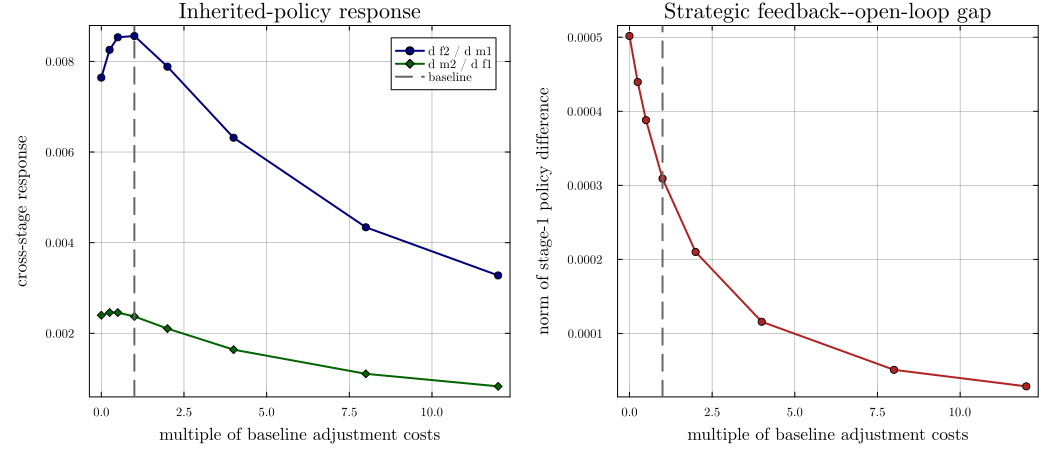
\includegraphics[width=0.94\textwidth]{adjustment_cost_sensitivity.png}
\caption{Two-stage strategic investment as primitive adjustment costs vary.}
\label{fig:sensitivity}
\end{figure}

This result clarifies the theoretical mechanism.  Adjustment costs make policy
a state, which is necessary for the particular lagged-instrument channel.
They do not ensure a large strategic motive.  The motive also requires
\begin{enumerate}
 \item a sizeable effect of current policy on a state observed in the next
       continuation game;
 \item a sizeable response of the rival's policy to that state; and
 \item a sizeable marginal effect of the rival's response on the investing
       authority's objective.
\end{enumerate}
The Australian baseline is weak primarily on the second and third margins.
The experiment therefore points toward transmission, mandate divergence, debt
exposure and shock persistence as the economically relevant sensitivity axes.

\section{Relation to fiscal dominance}

The model contains a strategic-debt channel but not a full fiscal-theory price-
level mechanism.  Fiscal expansion raises debt; debt is persistent; and both
future policy rules respond to debt.  Fiscal policy can therefore select a
future state that induces monetary accommodation or tightening.  This is close
to the strategic debt management mechanism in \citet{BeetsmaBovenberg1997}
and to the dynamic conflict studied by \citet{Tabellini1986}.

Fiscal dominance in the stronger sense concerns the inability or unwillingness
of monetary policy to stabilise prices without fiscal backing.  Nesting that
literature fully requires nominal government liabilities, a consolidated
intertemporal budget constraint and an explicit active/passive policy
classification.  The present model should therefore be interpreted as
capturing one strategic route toward fiscal pressure, rather than as a complete
fiscal theory of the price level.

The strategy-space result of \citet{Gnocchi2013} is especially relevant.  An
unrestricted monetary commitment can alter fiscal incentives in ways a simple
interest-rate path cannot.  In the present language, an open-loop path, a
Markov feedback rule and an institutionally committed rule are different
objects.  The game over adjustment coefficients belongs to the last category
and should be studied separately from policy-state investment.

\section{Steady state, shocks and coordination}

With zero gaps and no shocks, $s=0$ and $(m,f)=(0,0)$ form the common steady
state.  The realised strategic-investment wedge is then zero because every
quadratic marginal loss is zero.  This does not eliminate the game: the policy
derivatives in Table \ref{tab:twostage} remain features of the continuation
rules.  A shock moves the system away from the steady state and activates the
latent interaction.

Strategic complementarity should also be distinguished from equilibrium
multiplicity.  Positive cross responses can amplify policies while the joint
best-response system remains a contraction and the equilibrium remains unique.
Coordination on the ``right'' equilibrium becomes a separate issue when the
feedback mapping ceases to be contractive or the coupled Riccati system has
multiple stabilising solutions.  The baseline exhibits complementarity but
not numerical evidence of multiplicity.

\section{Limitations and the next structural extension}

Three limitations are important.  First, the empirical block is reduced form;
the private sector does not solve forward-looking Euler and pricing equations.
A structural extension should solve
\begin{align*}
 x_t&=E_tx_{t+1}-\sigma(m_t-E_t\pi_{t+1})+\psi f_t+d_t,\\
 \pi_t&=\beta E_t\pi_{t+1}+\kappa x_t+u_t
\end{align*}
jointly with the Markov policy rules.  Anticipated future policy would then
affect current activity and inflation, creating an additional commitment
channel.

Second, the local quadratic model cannot generate occasionally binding fiscal
limits, the effective lower bound or nonlinear debt-risk premia.  Those
features could enlarge strategic complementarities and create multiple
equilibria.  Third, the Australian exercise calibrates the debt block and
objectives.  Estimating the policy reaction and debt-transmission parameters
would be necessary before attaching empirical confidence intervals to the
strategic wedges.

\section{Conclusion}

The dynamic version of the two-stage game is a feedback Nash game in which
today's monetary and fiscal choices become tomorrow's state.  Backward
induction, not a separate game over objective coefficients, is the appropriate
extension.  The exact two-stage decomposition verifies a strategic-investment
motive in the Australian calibration.  Its magnitude is small, and that is an
informative result: adjustment costs establish durability, but the strategic
distortion is governed by the rival's response and by the investing authority's
valuation of that response.

The framework now supplies a disciplined foundation for the main research
question.  Stronger coordination problems should be sought by varying the
structural cross-effects, debt channel, mandate divergence and shock
persistence, and by checking for multiple stabilising feedback equilibria.
The fully forward-looking New Keynesian version is the natural next step.

\appendix
\section{Reproduction and numerical checks}

All calculations are in Julia.  From the parent
\texttt{australian\_four\_equation\_game} directory, run
\begin{verbatim}
julia --project=. dynamic_two_stage/run_dynamic_game.jl
julia --project=. dynamic_two_stage/build_tex.jl
\end{verbatim}
The first command recreates all CSV files, figures and numerical \LaTeX\
macros.  The second compiles this paper with the artifact-pinned Tectonic
binary.  The implementation checks the invertibility of every stage response
system, records open-loop condition numbers, verifies closed-loop stability and
runs the stationary fixed-point calculation from six initial value scales.

\begin{thebibliography}{99}

\bibitem[Beetsma and Bovenberg(1997)]{BeetsmaBovenberg1997}
Beetsma, R. M. W. J. and A. L. Bovenberg (1997).
Central bank independence and public debt policy.
\emph{Journal of Economic Dynamics and Control} 21, 873--894.
\url{https://doi.org/10.1016/S0165-1889(97)00003-1}.

\bibitem[Bulow, Geanakoplos and Klemperer(1985)]{BulowEtAl1985}
Bulow, J. I., J. D. Geanakoplos and P. D. Klemperer (1985).
Multimarket oligopoly: strategic substitutes and complements.
\emph{Journal of Political Economy} 93, 488--511.
\url{https://doi.org/10.1086/261312}.

\bibitem[Dixit(1980)]{Dixit1980}
Dixit, A. (1980).
The role of investment in entry-deterrence.
\emph{Economic Journal} 90, 95--106.
\url{https://doi.org/10.2307/2231658}.

\bibitem[Fudenberg and Tirole(1983)]{FudenbergTirole1983}
Fudenberg, D. and J. Tirole (1983).
Capital as a commitment: strategic investment to deter mobility.
\emph{Journal of Economic Theory} 31, 227--250.
\url{https://doi.org/10.1016/0022-0531(83)90075-3}.

\bibitem[Fudenberg and Tirole(1984)]{FudenbergTirole1984}
Fudenberg, D. and J. Tirole (1984).
The fat-cat effect, the puppy-dog ploy, and the lean and hungry look.
\emph{American Economic Review Papers and Proceedings} 74, 361--366.

\bibitem[Gnocchi(2013)]{Gnocchi2013}
Gnocchi, S. (2013).
Monetary commitment and fiscal discretion: the optimal policy mix.
\emph{American Economic Journal: Macroeconomics} 5, 187--216.
\url{https://doi.org/10.1257/mac.5.2.187}.

\bibitem[McKibbin(1987)]{McKibbin1987}
McKibbin, W. J. (1987).
Numerical solution of rational expectations models with and without strategic
behaviour. Reserve Bank of Australia Research Discussion Paper 8706.
\url{https://www.rba.gov.au/publications/rdp/1987/8706/}.

\bibitem[Oudiz and Sachs(1984)]{OudizSachs1984}
Oudiz, G. and J. D. Sachs (1984).
International policy coordination in dynamic macroeconomic models.
NBER Working Paper 1417.
\url{https://doi.org/10.3386/w1417}.

\bibitem[Reserve Bank of Australia(2026)]{RBAData}
Reserve Bank of Australia (2026).
Statistical tables.
\url{https://www.rba.gov.au/statistics/tables/}.

\bibitem[Tabellini(1986)]{Tabellini1986}
Tabellini, G. (1986).
Money, debt and deficits in a dynamic game.
\emph{Journal of Economic Dynamics and Control} 10, 427--442.
\url{https://doi.org/10.1016/S0165-1889(86)80001-X}.

\end{thebibliography}

\end{document}
